\documentclass[a4paper,12pt]{article}
\usepackage{amssymb}
\usepackage{amsmath}
\usepackage{graphicx}
\begin{document}
\title{Machine Learning Problem Set 2}
\author{Travis S. Collier, Graduate Student}
\date{2 October 2019}
\maketitle

\section{Problem 1}
I will solve the problem for $\sigma_c(x) = \frac{1}{1+e^{-cx}}$ and at the end specialize the result for $c=1$ \\
$\sigma_c(x) = \frac{1}{1+e^{-cx}} \Rightarrow \sigma^{'}_c(x) = \frac{ce^{-cx}}{(1+e^{-cx})^2}$\\
One notices immediately that $\sigma^{'}_c(x) = \sigma^{'}_c(-x) \therefore \sigma^{'}_c(x)$ is an even function symmetric about it's critical point at zero.\\
since $\sigma^{'}_c(x)$ is even we may evaluate it's behavior at $x=0$ and as $x\rightarrow\infty$\\
$\lim_{x\rightarrow\infty}\sigma^{'}_c(x) = \lim_{x\rightarrow\infty}\frac{ce^{-cx}}{(1+e^{-cx})^2} = 0$\\
At $x=0, \frac{ce^{-cx}}{(1+e^{-cx})^2}=\frac{c}{4}$ This is obviously the global maximum of the function since it has one inflection point and goes to 0 as $x\rightarrow\infty$\\
$\therefore 0 < \sigma^{'}_c(x) \leq \frac{c}{4}$\\
for $c=1$ this inequality becomes: $0 < \sigma^{'}(x) \leq \frac{1}{4}$\\

\section{Problem 2}
\begin{equation}
S(x)=
\begin{cases}
-1, &\text{if  }  x < 0,\\
1, &\text{if  }  x \geq 0
\end{cases}
\end{equation}
\begin{equation}
H(x)=
\begin{cases}
0, &\text{if  }  x < 0,\\
1, &\text{if  }  x \geq 0
\end{cases}
\end{equation}
\begin{equation}
ReLU(x)=xH(x)
\begin{cases}
0, &\text{if  }  x < 0,\\
x, &\text{if  }  x \geq 0
\end{cases}
\end{equation}

\subsection{Problem 2 a}
Show $S(x) = 2H(x)-1$\\
We proceed directly:\\
$2H(x) =$
$$
\begin{cases}
0, &\text{if  }  x < 0,\\
2, &\text{if  }  x \geq 0
\end{cases}
$$
$2H(x) - 1 =$
$$
\begin{cases}
-1, &\text{if  }  x < 0,\\
1, &\text{if  }  x \geq 0
\end{cases}
$$
This is $S(x)$\\
$\therefore S(x)=2H(x)-1$

\subsection{Problem 2 b}
Show $ReLU(x) = \frac{x}{2}(S(x)+1)$\\
We proceed directly:\\
$S(x)+1=$
$$
\begin{cases}
0, &\text{if  }  x < 0,\\
2, &\text{if  }  x \geq 0
\end{cases}
$$
$\frac{x}{2}(S(x)+1) =$\\
$$
\begin{cases}
0, &\text{if  }  x < 0,\\
x, &\text{if  }  x \geq 0
\end{cases}
$$
$\therefore ReLU(x) = \frac{x}{2}(S(x)+1)$


\section{Problem 3}
\subsection{3a}
For $sp(x)=ln(1+e^x)$ show $sp^{'} = \sigma(x)$\\
$\frac{d(ln(1+e^x)}{dx}=\frac{e^x}{1+e^x}$ (Using elementary derivative rules).\\
$\frac{e^x}{1+e^x} = \frac{1}{1+e^{-x}}$ (dividing by $e^x$ in all terms).\\
$\therefore sp^{'} = \frac{1}{1+e^{-x}}$
\subsection{3b}
$y=ln(1+e^x)$\\
$x=ln(1+e^y)$\\
$e^x=1+e^y$\\
$e^x-1=e^y$\\
$ln(e^x-1)= sp^{-1}(x)$\\
\subsection{3c}
$sp(x)=ln(1+e^x)$\\
$sp^{'}(x) = \frac{1}{1+e^{-x}}$,  $sp^{'}(-x) = \frac{e^{-x}}{1+e^{-x}}$\\
$sp^{'}(x) + sp^{'}(-x) = \frac{1}{1+e^{-x}} + \frac{e^{-x}}{1+e^{-x}}$\\
$sp^{'}(x) + sp^{'}(-x) = \frac{1+e^{-x}}{1+e^{-x}}$\\
$sp^{'}(x) + sp^{'}(-x) = 1$\\
$\sigma(x) + \sigma(-x) = 1$\\
$\sigma(x) = 1 - \sigma(-x)$\\


\section{Problem 4}
The Softsign function $so(x)$ is a continuous once differentiable function from $\mathbb{R}$ to the the interval $[-1,1]$ such that $so(x)=\frac{x}{1+|x|}$

\subsection{Problem 4 a}
Show that $so(x)$ is increasing.\\
The proof is direct.\\
Since $so(x)$ is differentiable we shall compute its derivative and show that it is positive everywhere which is the definition of increasing.\\
$\frac{d(\frac{x}{1+|x|}}{dx} = \frac{1}{(1+|x|)^2}$\\
This function is obviously strictly positive since it is the quotient of two positive functions.\\
Since the derivative is always positive the function is increasing by definition.

\subsection{Problem 4 b}
Prove that $so(x)$ is onto the interval $[-1,1]$.\\
Since $so(x)$ is continous, increasing, and bounded on the interval $[-1,1]$ we can employ the Intermediate Value Theorem.\\
$\forall r \in [-1,1] \exists x \in \mathbb{R} s.t. so(x) = r$ (Application of IVM)\\
This is also the definition of a function being surjective.\\
$\therefore so(x)$ is onto the interval $[-1,1]$.\\

\subsection{Problem 4 c}
Prove that $so(x)$ has inverse $so^{-1}(x) \forall x \in \mathbb{R}$ s.t. $|x| <1$\\
We will apply the elementary method to find the inverse:\\
Start with $so(x) =\frac{x}{1+|x|}$ and commute $so(x)\leftrightarrow x$ and rename $so(x)\rightarrow so^{-1}(x)$
$x =\frac{so^{-1}}{1+|so^{-1}|}$
$x(1+|so^{-1}|) = so^{-1}$
$x = so^{-1} - |x|so^{-1}$
We now constrict to the domain  $|x| <1 so we may divide$\\
$\frac{x}{1-|x|} =so^{-1}(x)$

\subsection{Problem 5}
Show $S(y_i) = \frac{e^{y_i}}{\sum_{j}e^{y_j}}$ is invariant by translation by a constant vector.\\
Let c be the value of the constant vector such that $S(y_i + c) = \frac{e^{y_i + c}}{\sum_{j}e^{y_j + c}}$\\
$S(y_i + c) = \frac{e^{y_i }e^c}{\sum_{j}e^{y_j}e^c}$ (Elementary properties of exp)\\
$S(y_i + c) = \frac{e^{y_i }}{\sum_{j}e^{y_j}}$\\
$S(y_i + c) = S(y_i)$\\

\subsection{Problem 6}
This python code will produce the softsign function and it's inverse and plot them (The data\_softsign is capped at $|x|=.8$ to make the graph intelligible.)\\
import numpy as np\\
import matplotlib.pyplot as plt\\
\\
def SoftSign(data):\\
    output = data/(1+np.abs(data))\\
    return output\\
\\
def InvSoftSign(data):\\
    output = data/(1-np.abs(data))\\
    return output\\
\\
data\_softsign = np.linspace(-.8, .8, num=100000)\\
data = np.linspace(-1000.0, 1000.0, num=100000)\\
plt.plot(data,SoftSign(data))\\
plt.plot(data,InvSoftSign(data\_softsign))\\
plt.legend(['SoftSign','Inverse of SoftSign'])\\
plt.show()\\

\begin{figure}[h!]
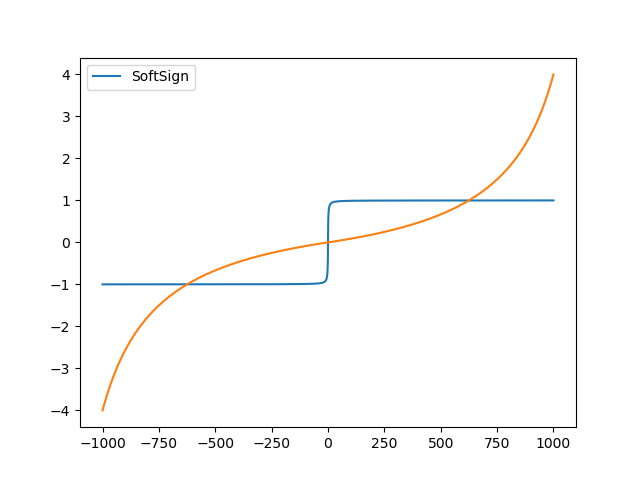
\includegraphics[width = .9\linewidth]{Figure_1}
\end{figure}



\end{document}